
WordNet \cite{Miller95wordnet:a} --- лексическая база данных английского языка, разработанная в Принстонском университете.
Она представляет собой электронный словарь-тезаурус и набор семантических сетей для английского языка.

Словарь, представленный в WordNet, состоит из 4 семантических сетей для основных знаменательных частей речи:
существительных, глаголов, прилагательных и наречий.

Этапы применения WordNet к модели, описанной в предыдущем разделе:
\begin{enumerate}[1)]
    \item провести грамматический разбор запроса, выявить части речи, соответствующие словам;
    \item определить (хотя бы приближенно) возможную семантику слова в соответствии с контекстом;
    \item найти с использованием WordNet похожие слова (согласно метрике семантической близости);
    \item ранжировать поисковую выдачу в соответствии с семантической близостью слов и $n$-грамм для
          последующего обучения нейронной сети (с помощью классических алгоритмов либо субъективно);
    \item обучить нейросеть и провести сравнение результатов.
\end{enumerate}

Семантическая близость $n$-грамм может быть определена как среднее геометрическое коэффициентов близости отдельных слов:
\begin{equation}
    \label{eq:ngram-sim}
    \begin{aligned}
        S(u_1u_2\dots u_n, w_1w_2\dots w_n) = \left( \prod\limits_{i=1}^n {S(u_i, w_i)} \right)^{\frac1n}= \\
        = \sqrt[n]{S(u_1, w_1)S(u_1, w_2)\dots S(u_n, w_n)},
    \end{aligned}
\end{equation}
где $u_1u_2\dots u_n$ и $w_1w_2\dots w_n$ --- сравниваемые $n$-граммы (здесь мы считаем, что порядок слов имеет значение).

Формула \eqref{eq:ngram-sim} может быть продиктована следующими соображениями:
\begin{enumerate}[1)]
    \item коэффициент близости должен равняться некоторому <<среднему>> из коэффициентов близости отдельных слов;
    \item с другой стороны, наличие неподобных пар слов должно приводить к значительному (но не полному) снижению
          близости всей $n$-граммы (что позволяет отсечь, например, среднее арифметическое).
\end{enumerate}

Одним из базовых методов для выведения семантики слова в контексте (разрешения неоднозначности, англ. disambiguation)
является метод Леска \cite{10.1145/318723.318728}, разработанный инженером компании Bell Labs М. Леском в 1986 году.
Идея метода заключается в поиске значения слова в списке словарных определений с учетом контекста, где это слово использовано.
Основным критерием для выбора значения послужило следующее правило: заложенный в этом определении смысл должен был частично
совпадать со смыслом значений соседних слов в контексте.

Алгоритм Леска работает в следующей последовательности:
\begin{enumerate}[1)]
    \item На первом шаге алгоритма отделяется контекст для рассматриваемого слова --- чаще всего, не более 10 расположенных
          рядом слов.
    \item Далее, для рассматриваемого слова (или его начальной формы) ищутся все определения в некоторой базе знаний
          (например, толковом словаре, хотя данный вариант редко используется непосредственно).
    \item Затем происходит поиск слов из контекста в каждом найденном определении. Если какое-либо слово из контекста
          присутствует в определении, то данное определение получает "<балл"> --- т. е. увеличивается счетчик совпадений.
    \item Наконец, происходит ранжирование определений по значениям счетчика совпадений. Чем выше значение счетчика, тем более
          подходящим к контексту считается определение.
\end{enumerate}

Рассмотрим следующий пример: согласно Большому толковому словарю русского языка С. А. Кузнецова \cite{kuznecov2008noveishiy},
слово "<штанга"> в русском языке имеет следующие значения:
\begin{enumerate}[1)]
    \item металлический стержень, используемый как деталь во многих механизмах;
    \item боковая стойка (иногда и верхняя перекладина) футбольных, хоккейных и т.п. ворот;
    \item снаряд для занятий тяжёлой атлетикой, состоящий из металлического стержня, на концах которого укреплены
          съёмные диски различного веса.
\end{enumerate}

Теперь рассмотрим следующие предложения, содержащие слово "<штанга">:
\begin{enumerate}[1)]
    \item Троллейбусная штанга, как правило, изготовляется из металлической трубы переменного сечения.
    \item В футбольном матче между "<Спартаком"> и "<Зенитом"> форвард ленинградцев дважды поразил штангу, а защитник москвичей
          отметился голом в свои ворота.
    \item На чемпионате мира по тяжелой атлетике наш спортсмен поднял штагу рекордного веса.
\end{enumerate}

Как видим, в первом предложении присутствует слово "<металлический">, которое есть только в первом определении слова "<штанга">.
Во втором предложении такую же роль играют слова "<футбольный"> и "<ворота">, в третьем --- "<вес"> и "<тяжелая атлетика">.
Таким образом, в данном примере алгоритм работает безупречно, правильно определяя значение слова в зависимости от контекста.

Чаще, к сожалению, возникает обратная ситуация --- а именно, когда словарное определение оказывается недостаточно емким и не включает
в себя наиболее часто встречающиеся в контексте слова. Поэтому чаще применяются модификации алгоритма, основанные не только на
словарных определениях, но и на примерах употребления слов в данных значениях в контексте.

Для применения алгоритма воспользуемся методом, содержащимся непосредственно в библиотеке NLTK. Он возвращает для заданного слова
в предложении наиболее подходящий (с точки зрения алгоритма) набор синонимов, иначе --- синонимический ряд (англ. synset),
представляющий из себя слова со схожим значением, объединенные в узел семантической сети. В WordNet каждый такой набор дополнен
определением и примерами употребления слов в контексте. Слова, имеющие несколько значений, включаются в несколько синонимических рядов
(выбор между которыми в контексте заданного поискового запроса или предложения будет осуществляться с помощью алгоритма Леска)
и могут быть причислены к различным синтаксическим и лексическим классам.

Синонимические ряды, в отличие от лишенных контекста слов, уже подлежат количественной оценке схожести.

В качестве метрики семантической близости воспользуемся метрикой Ву-Палмер \cite{10.3115/981732.981751}, предложенной в 1994 году
специалистами по компьютерной лингвистике Чжибяо Ву и Мартой Палмер. Она вычисляется по следующей формуле
\begin{equation}
    \label{eq:wup-sim}
    S_{WP} = 2\times\frac{d(\mathrm{LCS}(s_1, s_2))}{d(s_1) + d(s_2)}
\end{equation}
Здесь $d(s)$ --- глубина синонимического ряда $s$ в таксономии WordNet, $\mathrm{LCS}(s_1, s_2)$ --- наиболее специфический
(то есть, наименее общий) узел (англ. least common subsumer), являющийся предком как $s_1$, так и $s_2$.

Заметим, что метрика \eqref{eq:wup-sim} определена не всегда, поскольку таксономия может не быть деревом (в общем случае, это лес),
а значит, $\mathrm{LCS}(s_1, s_2)$ для произвольных $s_1$ и $s_2$ может не существовать. Однако же, в нашем случае, поскольку мы
во всех случаях вычисляем метрику подобия между схожими словами, имеющими общего предка в таксономии.

Если метрика \eqref{eq:wup-sim} определена, то всегда $0 < S_{WP}\leqslant 1$ (заметим, что она всегда строго больше 0, поскольку
глубина корня в таксономии по определению считается равной 1).

Для некоторых частей речи в WordNet (в частности, прилагательных и наречий) таксономия не организована в виде иерархии, поэтому
вычисление $S_{WP}$ становится невозможным. Наиболее простым подходом в таком случае является назначение таким парам синонимических
рядов константной метрики, то есть, фиксированного значения $0 < \alpha < 1$ (значение 1 используется только в случае, когда $s_1=s_2$,
то есть, слово считается максимально близко семантически самому себе). В нижеописанных экспериментах используется данный подход,
применяется значение $\alpha=0{,}2$.

Далее, нам необходимо модифицировать метрики TF-IDF \eqref{eq:norm-tf} и \eqref{eq:shifted-idf} для того, чтобы они учитывали вхождение
в тексты документов не только самих слов, но и их синонимов (включая семантическую близость). Наиболее естественным для этого представляется
подход с использованием взвешенного количества слов:

\begin{equation}
    \label{eq:adjusted-word-count}
    \tilde{N}_w(d) = \sum\limits_{s\in\mathrm{Syn}(w)} N_s(d) S_{WP}(w, s)
\end{equation}
Здесь $\tilde{N}_w(d)$ --- количество вхождений слова $w$ и его синонимов (с учетом близости) в документ $d$, $\mathrm{Syn}(w)$ --- множество
синонимов слова $w$ (подразумевается, что слово считается синонимом самого себя, т.е. $w\in\mathrm{Syn}(w)$ и $S_{WP}(w, w)=1$).

Заметим, что "<количество">, определенное по формуле \eqref{eq:adjusted-word-count}, может и не быть целым числом (что очевидно следует из
определения). Однако, это не влияет на корректность вычислений метрик TF-IDF по формулам \eqref{eq:norm-tf} и \eqref{eq:shifted-idf}.

\subsubsection{Источники текстовых документов и база данных}
В рассматриваемой модели использовались те же источники (см. стр. \pageref{lab:sources-grammar}) и та же база данных (стр. \pageref{lab:db-grammar}),
что и в модели на основе грамматической структуры текстов, рассмотренной в предыдущем разделе.

\subsubsection{Генеративно-состязательная сеть}
Помимо топологии генеративно-состязательной сети, использованной в предыдущей модели (см. стр. \pageref{lab:gan-grammar}), была использована модель с
с добавлением дополнительного слоя с 2048 нейронами. Структура всей сети выглядит следующим образом:
\begin{itemize}
    \item для подсети $G$:
          \begin{itemize}
              \item входной слой с размером 100 (для случайного
                    входа);
              \item слой с 256 нейронами, с использованием выпрямителя с протечкой при $\alpha = 0.2$;
              \item слой с 512 нейронами, с использованием выпрямителя с протечкой при $\alpha = 0.2$;
              \item слой с 1024 нейронами, с использованием выпрямителя с протечкой при $\alpha = 0.2$;
              \item слой с 2048 нейронами, с использованием выпрямителя с протечкой при $\alpha = 0.2$;
              \item выходной слой с размером 32, использующий гиперболический тангенс в качестве функции активации.
          \end{itemize}
    \item для подсети $D$:
          \begin{itemize}
              \item входной слой с размером 32 (для подачи векторов параметров, генерируемых подсетью G);
              \item слой с 2048 нейронами, использующий ReLU с $\alpha = 0.2$;
              \item слой отсева с коэффициентом 0,3;
              \item слой с 1024 нейронами, использующий ReLU с $\alpha = 0.2$;
              \item слой отсева с коэффициентом 0,3;
              \item слой с 512 нейронами, использующий ReLU с $\alpha = 0.2$;
              \item слой отсева с коэффициентом 0,3;
              \item слой с 256 нейронами, использующий ReLU с $\alpha = 0.2$;
              \item слой отсева с коэффициентом 0,3;
              \item выходной слой с размерностью 1 (скалярное значение, обозначающее оценку релевантности).
          \end{itemize}
\end{itemize}

\subsubsection{Полученные результаты}
Результаты для обеих конфигураций генеративно-состязательных сетей представлены в таблицах \ref{tab2} и \ref{tab3}, а также на рис. \ref{fig:wn-scores-1}.
\begin{table}[tbp]
    \caption{Результаты поисковых запросов в модели с 3 слоями}
    \begin{center}
        \begin{tabular}{ccc}
            \toprule
            \textbf{Запрос}                           & \multicolumn{2}{c}{\textbf{Оценка релевантности}}                               \\
                                                      & \textbf{\textit{Top 10}}                          & \textbf{\textit{Bottom 10}} \\
            \midrule
            india  fifteen minutes more he passed     & \(\mu=0.6021\)                                    & \(\mu=0.3059\)              \\
                                                      & \(\sigma=0.2263\)                                 & \(\sigma=0.0312\)           \\
            \midrule
            that he had also seen her                 & \(\mu=0.8491\)                                    & \(\mu=0.2677\)              \\
                                                      & \(\sigma=0.0158\)                                 & \(\sigma=0.3058\)           \\
            \midrule
            more serious than by you do know          & \(\mu=0.8759\)                                    & \(\mu=0.1647\)              \\
                                                      & \(\sigma=0.0506\)                                 & \(\sigma=0.0233\)           \\
            \midrule
            answer that he asked questions to come to & \(\mu=0.8948\)                                    & \(\mu=0.8529\)              \\
                                                      & \(\sigma=0.0080\)                                 & \(\sigma=0.0506\)           \\
            \midrule
            was a bull turned from sam                & \(\mu=0.8709\)                                    & \(\mu=0.5615\)              \\
                                                      & \(\sigma=0.0355\)                                 & \(\sigma=0.3926\)           \\
            \midrule
            likely place that was with such matters   & \(\mu=0.7994\)                                    & \(\mu=0.3423\)              \\
                                                      & \(\sigma=0.1651\)                                 & \(\sigma=0.3689\)           \\
            \midrule
            and when i tried to the greatest          & \(\mu=0.9092\)                                    & \(\mu=0.8777\)              \\
                                                      & \(\sigma=0.0236\)                                 & \(\sigma=0.0165\)           \\
            \midrule
            i knew una had wept  he                   & \(\mu=0.6551\)                                    & \(\mu=0.3681\)              \\
                                                      & \(\sigma=0.1944\)                                 & \(\sigma=0.0360\)           \\
            \bottomrule
        \end{tabular}\label{tab2}
    \end{center}
\end{table}
\begin{table}[tbp]
    \caption{Результаты поисковых запросов в модели с 4 слоями}
    \begin{center}
        \begin{tabular}{ccc}
            \toprule
            \textbf{Запрос} & \multicolumn{2}{c}{\textbf{Оценка релевантности}}                               \\
                            & \textbf{\textit{Top 10}}                          & \textbf{\textit{Bottom 10}} \\
            \midrule
            then true for its sake on himself         & \(\mu=0.6028\)                                    & \(\mu=0.0888\)              \\
                                                      & \(\sigma=0.3811\)                                 & \(\sigma=0.0567\)           \\
            \midrule
            she answered   presently i said           & \(\mu=0.8736\)                                    & \(\mu=0.0272\)              \\
                                                      & \(\sigma=0.0147\)                                 & \(\sigma=0.0028\)           \\
            \midrule
            within hollow her large eyes large full   & \(\mu=0.4586\)                                    & \(\mu=0.0408\)              \\
                                                      & \(\sigma=0.4197\)                                 & \(\sigma=0.0049\)           \\
            \midrule
            how you did  i have been                  & \(\mu=0.5236\)                                    & \(\mu=0.0110\)              \\
                                                      & \(\sigma=0.4211\)                                 & \(\sigma=0.0019\)           \\
            \midrule
            other but he found his courage at least   & \(\mu=0.8612\)                                    & \(\mu=0.6925\)              \\
                                                      & \(\sigma=0.0046\)                                 & \(\sigma=0.1937\)           \\
            \midrule
            my life very that was than ever           & \(\mu=0.7160\)                                    & \(\mu=0.2305\)              \\
                                                      & \(\sigma=0.3386\)                                 & \(\sigma=0.3608\)           \\
            \midrule
            deem  remember that he was interests      & \(\mu=0.7913\)                                    & \(\mu=0.3335\)              \\
                                                      & \(\sigma=0.1954\)                                 & \(\sigma=0.2972\)           \\
            \midrule
            oh don  your true taste white             & \(\mu=0.1604\)                                    & \(\mu=0.0718\)              \\
                                                      & \(\sigma=0.1300\)                                 & \(\sigma=0.0042\)           \\
            \bottomrule
        \end{tabular}\label{tab3}
    \end{center}
\end{table}

\begin{figure}
    \centerline{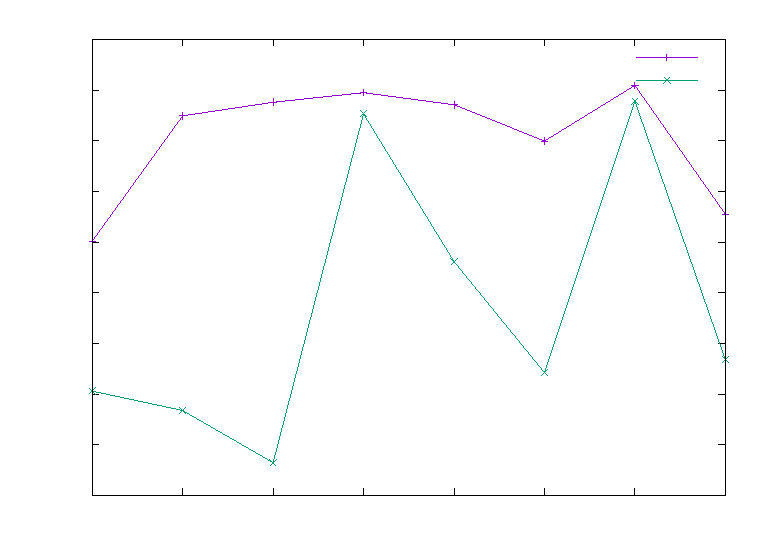
\includegraphics[scale=0.8]{312-1_scores.eps}}
    \caption{Оценки релевантности для модели с 3 слоями}\label{fig:wn-scores-1}
\end{figure}

\begin{figure}
    \centerline{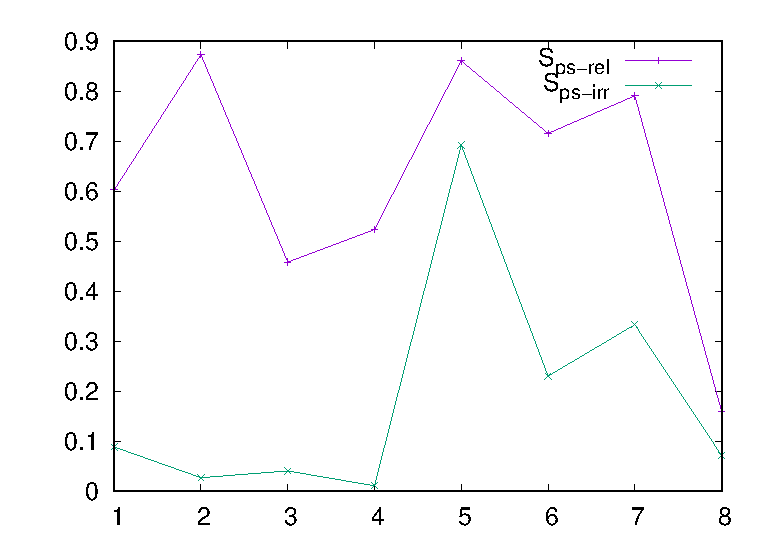
\includegraphics[scale=0.8]{312-2_scores.eps}}
    \caption{Оценки релевантности для модели с 4 слоями}\label{fig:wn-scores-2}
\end{figure}

Заметим, что при использовании обеих топологий прослеживается четкая грань между псевдорелевантными и псевдонерелевантными результатами поисковой выдачи.
Следует также заметить, что сравнение абсолютных оценок релевантности для разных запросов смысла не имеет, важны лишь относительные оценки для каждого 
конкретного запроса в отдельности (поскольку при ранжировании результатов каждый запрос обрабатывается по отдельности, а выдача ранжируется (сортируется)
в соответствии со значением оценки, которе используется лишь для определения позиции (ранга) результата в выдаче по запросу).

На основании полученных результатов мы можем сразу же выявить преимущества и недостатки модели,
основанной на WordNet, по сравнению с простейшей моделью, учитывающей лишь грамматические словоформы:
\begin{itemize}
    \item увеличился охват запросов документами, в связи с тем, что, в отличие от предыдущей модели, в рассматриваемой
          учитываются не только сами слова, входящие в запрос, но и семантически близкие им. Это в некоторых случаях позволило
          увеличить точность запросов и релевантность результатов, что показало больший разброс в поисковой выдаче и дало
          возможность продемонстрировать различия в псевдорелевантных и псевдонерелевантных результатах;
    \item с другой стороны, контекст запроса часто не позволяет однозначно определить семантику того или иного слова 
          в типологии WordNet. В частности, в ходе подготовки данных для моделей и отладки написанных программ было
          выяснено, что в ходе применения алгоритма Леска для часто распространенных английских слов I (я) и as (союз "<как">)
          в качестве синонимов часто упоминались слова indium (индий) и arsenic (мышьяк). Это связано с символами I и As для
          соответствующих химических элементов --- индия и мышьяка, которые практически во всех случаях не имели реального
          отношения к запросу;
    \item WordNet не позволяет опредлить на уровне метрики подобие некоторых частей речи (в частности, прилагательных), но применение
          константного значения для пар синонимических рядов с неопределенной метрикой нельзя считать исчерпывающим решением проблемы,
          поскольку прилагательные также могут иметь неравноценные синонимы.
\end{itemize}
В целом, WordNet является базой знаний для текстов общего назначения, поэтому ее применение к специализированным корпусам текстов 
(специализация пространства поиска) не всегда может давать лучшие результаты (поэтому перспективным представляется использование модели,
описанной в следующем разделе, поскольку она может быть обучена на исходных данных того же характера, что и входящие в пространство поиска 
(включая сами данные из пространства поиска)). Подводя итог сказанному, можем заключить, что модель с использованием WordNet имеет как
свои преимущества, так и недостатки по сравнению с простейшей моделью, однако путем грамотного и обоснованного подбора баз знаний (в частности,
таксономий типа WordNet) и настройки параметров можно добиться улучшения результатов и использования всех преимуществ WordNet (следует, однако,
заметить, что процесс этот требудет значительного объема "<ручного"> (то есть, неавтоматизируемого, требующего серьезного вмешательства человека) труда,
что не во всех случаях является лучшим решением).